\section{The Analysis Strategy}

The most important aspect of any SUSY analysis is the methodology used to estimate the background contribution in the signal region. The first step consists in the determination of all the main background sources and the definition of an estimation technique for each of the contributions. 

In the Standard Model, all small processes leading to like-sign di-$\hadtau$ final states have small cross sections. On the other hand production of QCD events in a hadron collider has large cross sections. Therefore, even small fake jet-$\hadtau$ fake rates from QCD processes, matter. Also, in QCD events, additional jet activity from initial or final jet radiation processes is expected, which gives these type of events a high probability to pass the VBF selection criteria. Those motivations lead to the determination of QCD as main background source for this analysis. 

The Monte Carlo simulation of QCD events is not reliable due to the complicated modeling of the interactions at the partonic level and the complex fragmentation processes of the resulting jets. Therefore the decision to use a data-driven approach. The number of QCD events in signal region (SR) is estimated directly from data from a defined control region (CR) using the proper correction factor. This correction factor can be properly measured in other exclusive control regions. 

The following formula gives a simple description of the whole methodology:

\begin{equation}
N^{QCD}_{SR} =  N^{DATA}_{CR} * CF
\label{eq:qcdbgpred_simple}
\end{equation} 

where $N^{QCD}_{SR}$ is the number of QCD events predicted in the signal region, $N^{DATA}_{CR}$ is the number of data events in the control region and CF is the correction factor. 

Four other types of background contributions has been considered in this analysis. 

Further details on the event selection, the  data-driven method and the control regions definition is given in the next section. 

The first irreducible background contribution is coming from the Standard Model VBF processes resulting in two \hadtau and two jets as shown in Figure \ref{fig:background_SMVBF}. This background contribution is well modeled being purely electroweak and its cross section is very small. Therefore this  background is considered minor and its contribution is directly taken from simulation.

\begin{figure}[tbh!]
	\centering
	\begin{tabular}{cc}
		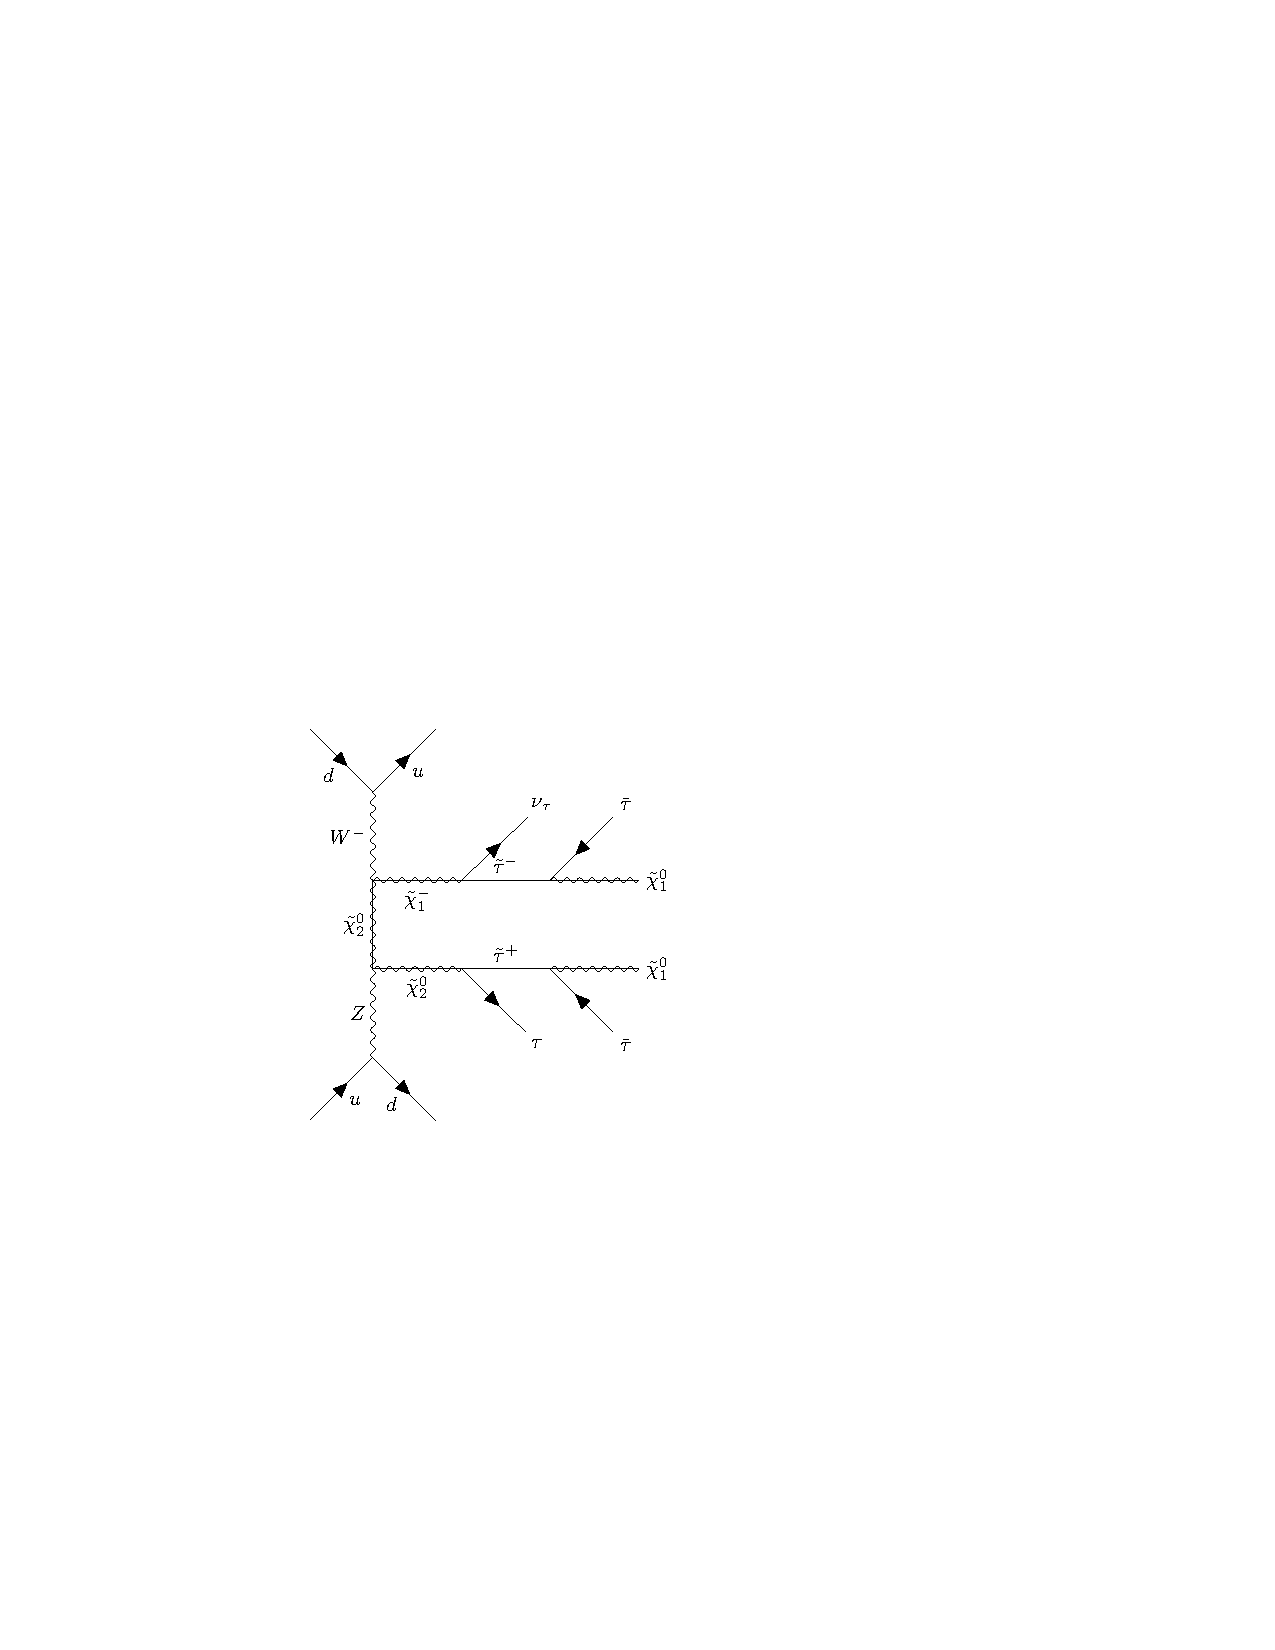
\includegraphics[width=0.50\textwidth]{diagrams/pics/signal_C1N2.pdf}
		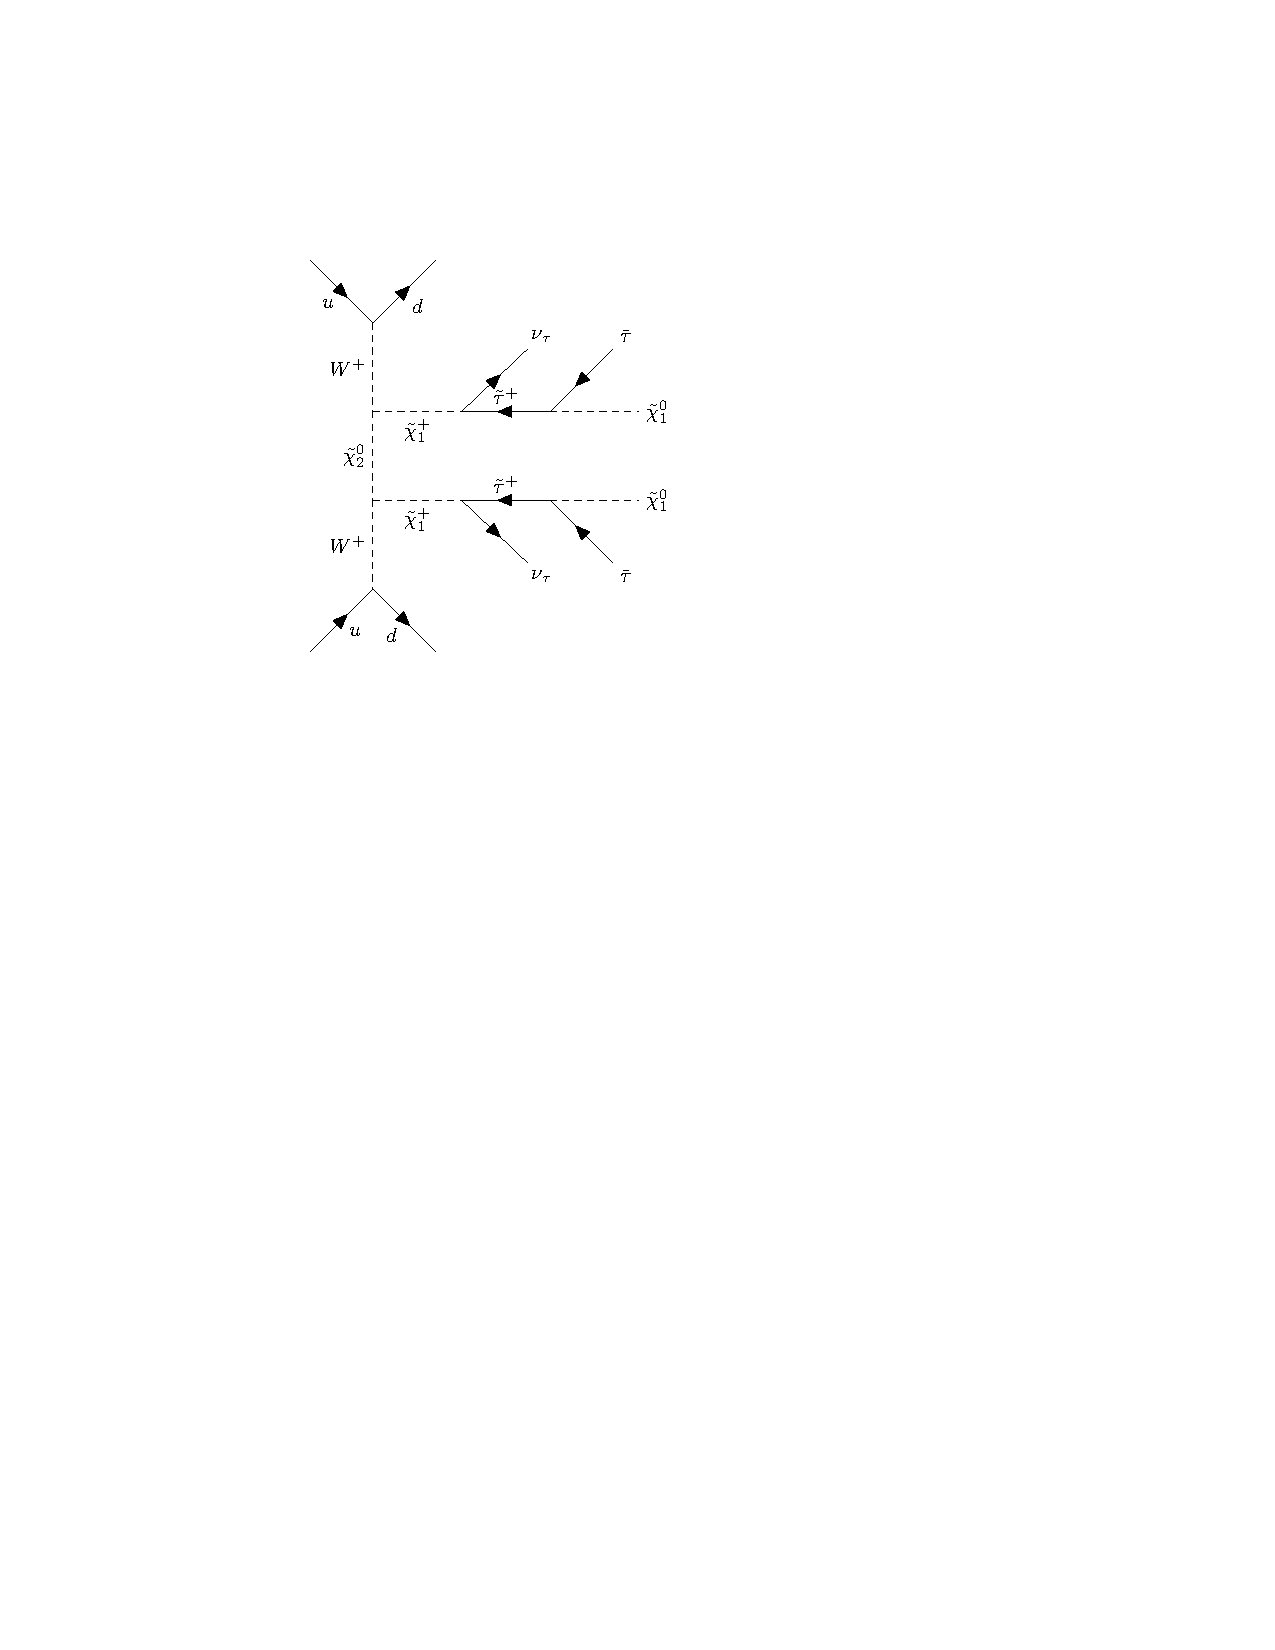
\includegraphics[width=0.50\textwidth]{diagrams/pics/signal_C1C1.pdf} 		
	\end{tabular}
	\caption{Diagrams of (left) \charginopm \neutralinotwo and (right) \charginopm \charginomp pair production through vector-boson fusion followed by their decays to $\tau$ leptons and the LSP.}
	\label{fig:background_SMVBF}
\end{figure}

\clearpage
\subsection{Monte Carlo Samples}

\begin{table}[ht]
	\tiny
	\centering{
		\begin{tabular}{| l | l |}
			\hline
			&\\
				Process &Official CMS Datasets /DY*/AODSIM \\
			&\\
				\hline		
				&\\
				$Z \longrightarrow \tau\tau$ & \texttt{ToTauTau\_M-20\_CT10\_TuneZ2star\_v2\_8TeV-powheg-tauola-pythia6/Summer12 DR53X-PU\_S10\_START53\_V7A-v2} \\
				&\\
				$Z \longrightarrow \mu\mu$ & \texttt{ToMuMu\_M-20\_CT10\_TuneZ2star\_v2\_8TeV-powheg-pythia6/Summer12\_DR53X-PU\_S10\_START53\_V7A-v1} \\
				&\\
				$Z \longrightarrow ee$ & \texttt{ToEE\_M-20\_CT10\_TuneZ2star\_v2 8TeV-powheg-pythia6/Summer12\_DR53X-PU\_S10\_START53 V7A-v1} \\
				&\\
				$Z \longrightarrow ll~(10 < m_{ll} < 50)$ & \texttt{JetsToLL\_M-10To50\_TuneZ2Star\_8TeV-madgraph/Summer12\_DR53X-PU\_S10\_START53\_V7A-v1} \\
				&\\
				$Z \longrightarrow ll~(m_{ll} > 50)$ & \texttt{JetsToLL\_M-50\_TuneZ2Star\_8TeV-madgraph-tarball/Summer12\_DR53X-PU\_S10 START53\_V7A-v1} \\
				&\\
				$Z \longrightarrow ll + 1jets$ &
				\texttt{1JetsToLL\_M-50\_TuneZ2Star\_8TeV-madgraph/Summer12\_DR53X-PU\_S10 START53\_V7A-v1} \\
				&\\
				$Z \longrightarrow ll + 2jets$ & \texttt{2JetsToLL\_M-50\_TuneZ2Star\_8TeV-madgraph/Summer12\_DR53X-PU\_S10\_START53\_V7A-v1} \\
				&\\
				$Z \longrightarrow ll + 3jets$ &
				\texttt{3JetsToLL\_M-50\_TuneZ2Star\_8TeV-madgraph/Summer12 DR53X-PU\_S10\_START53\_V7A-v1} \\
				&\\
				$Z \longrightarrow ll + 4jets$ &
				\texttt{4JetsToLL\_M-50\_TuneZ2Star\_8TeV-madgraph/Summer12 DR53X-PU\_S10\_START53\_V7A-v1} \\
				&\\
				$Z \longrightarrow ll~EWK$ &
				\texttt{JJ01JetsToLL\_M-50\_MJJ-200\_TuneZ2Star 8TeV-madgraph\_tauola/Summer12\_DR53X-PU\_S10 START53\_V7A-v1} \\
				&\\
				\hline
		\end{tabular}
	}
	\caption{ Drell Yang simulated samples.}
	\label{teble:samples_DY} % is used to refer this table in the text
\end{table}

\begin{table}[ht]
	\tiny
	\centering{
		\begin{tabular}{| l | l |}
			\hline
			&\\
			Process &Official CMS Datasets /W*/AODSIM \\
			&\\
			\hline		
			&\\
W + 0 jets & \texttt{JetsToLNu\_TuneZ2Star\_8TeV-madgraph-tarball/Summer12\_DR53X-PU\_S10 START53\_V7A-v2} \\
&\\
W + 1 jet & \texttt{1JetsToLNu\_TuneZ2Star\_8TeV-madgraph/Summer12\_DR53X-PU\_S10\_START53\_V7A-v1} \\
&\\
W + 2 jets & \texttt{2JetsToLNu\_TuneZ2Star\_8TeV-madgraph/Summer12\_DR53X-PU\_S10\_START53\_V7A-v1} \\
&\\
W + 3 jets &
\texttt{3JetsToLNu\_TuneZ2Star\_8TeV-madgraph/Summer12\_DR53X-PU\_S10 START53\_V7A-v1} \\
&\\
W + 4 jets & \texttt{4JetsToLNu\_TuneZ2Star\_8TeV-madgraph/Summer12\_DR53X-PU\_S10\_START53\_V7A-v1} \\
			&\\
			\hline
		\end{tabular}
	}
	\caption{ W boson plus additional jets simulated samples.}
	\label{teble:samples_Wjets} % is used to refer this table in the text
\end{table}

\begin{table}[ht]
	\tiny
	\centering{
		\begin{tabular}{| l | l |}
			\hline
			&\\
			Process &Official CMS Datasets /TTJets*/AODSIM \\
			&\\
			\hline		
			\ttbar & \texttt{MassiveBinDECAY\_TuneZ2star\_8TeV-madgraph-tauola/Summer12\_DR53X-PU\_S10\_START53\_V7C-v1} \\
			&\\
			
			&\\
			\hline
		\end{tabular}
	}
	\caption{Standard model top production simulated sample.}
	\label{teble:samples_ttbar} % is used to refer this table in the text
\end{table}

\begin{table}[ht]
	\tiny
	\centering{
		\begin{tabular}{| l | l |}
			\hline
			&\\
			Process &Official CMS Datasets */AODSIM \\
			&\\
			\hline		
			&\\
			$WW(\longrightarrow 2l2\nu)$ & \texttt{WJetTo2L2Nu\_8TeV-powheg-pythia6/Summer12\_DR53X-PU\_S10\_START53\_V7C-v1} \\
			&\\
			$W^{+}W^{+}$ & \texttt{/WpWpqq\_8TeV-madgraph/Summer12\_DR53X-PU\_S10\_START53\_V7A-v1} \\
			&\\
			$W^{−}W^{−}$ & \texttt{/WmWmqq\_TeV-madgraph/Summer12\_R53X-PU\_10\_START53\_V7A-v1} \\
			&\\
			WW double scattering & \texttt{/WW\_DoubleScattering\_8TeV-pythia8/Summer12\_DR53X-PU\_S10\_START53\_V7A-v1} \\
			&\\
			WW EWK & \texttt{/WWjjTo2L2Nu\_8TeV\_madgraph\_qed6\_qcd0/Summer12\_DR53X-PU\_S10\_\_V19-v1} \\
			&\\
			$WZ~(\longrightarrow 2q2\nu)$ & \texttt{/WZJetsTo2Q2Nu\_TuneZ2star\_8TeV-madgraph-tauloa/Summer12\_DR53X-PU\_S10\_START53\_V7A-v1} \\
			&\\
			$WZ~(\longrightarrow 2l2\nu)$ & \texttt{/WZJetsTo2L2Nu\_TuneZ2star\_8TeV-madgraph-tauloa/\_DR53X-PU\_S10\_START53\_V7A-v1} \\
			&\\
			$WZ~(\longrightarrow 3l)$ & \texttt{/WZJetsTo3L\_TuneZ2star\_8TeV-madgraph-tauloa/Summer12\_DR53X-PU\_S10 START53\_V7A-v1} \\
			&\\
			$ZZ~(\longrightarrow 2q2\nu)$ & \texttt{/ZZJetsTo2Q2Nu\_TuneZ2star\_8TeV-madgraph-tauloa/Summer12\_DR53X-PU\_S10\_START53\_V7A-v1} \\
			&\\
			$ZZ~(\longrightarrow 2l2\nu)$ & \texttt{/ZZJetsTo2L2Nu\_TuneZ2star\_8TeV-madgraph-tauloa/Summer12\_DR53X-PU\_S10\_START53\_V7A-v1} \\
			&\\
			$ZZ~(\longrightarrow 2l2q)$ & \texttt{/ZZJetsTo2L2Q\_TuneZ2star\_8TeV-madgraph-tauloa/Summer12\_DR53X-PU\_S10\_START53\_V7A-v1} \\
			&\\
			$ZZ~(\longrightarrow 4l)$ & \texttt{/ZZJetsTo4L\_TuneZ2star\_8TeV-madgraph-tauloa/Summer12\_DR53X-PU\_S10\_START53\_V7A-v1} \\

			&\\
			\hline
		\end{tabular}
	}
	\caption{ Standard model production of two vector bosons simulated samples.}
	\label{teble:samples_VV} % is used to refer this table in the text
\end{table}

\begin{table}[ht]
	\tiny
	\centering{
		\begin{tabular}{| l | l |}
			\hline
			&\\
			Process &Official CMS Datasets /VBF */AODSIM \\
			&\\
			\hline
			&\\
			$H \longrightarrow WW(\longrightarrow 2l)$ & \texttt{HToWWTo2LAndTau2Nu\_M-125\_8TeV-powheg-pythia6/Summer12\_DR53X-\_S10\_START53\_V7A-v1} \\
			&\\
			$H \longrightarrow ZZ(\longrightarrow 2l2\nu)$ & \texttt{HToZZTo2L2Nu\_M-120\_8TeV-powheg-pythia6/Summer12\_DR53X-PU\_S10\_START53\_V7A-v1} \\
			&\\
			$H \longrightarrow ZZ~(\longrightarrow 2l2q)$ & \texttt{HToZZTo2L2Q\_M-125\_8TeV-powheg-pythia6/Summer12\_DR53X-PU\_S10\_START53\_V7A-v1} \\
			&\\
			$H \longrightarrow ZZ~(→ 4l)$ & \texttt{HToZZTo4L\_M-125\_8TeV-powheg-pythia6/Summer12\_DR53X-PU\_S10\_START53\_V7A-v1} \\
			&\\
			$H \longrightarrow ZZ~(\longrightarrow 4\nu)$ & \texttt{HToZZTo4Nu\_M-120\_8TeV-pythia6/Summer12\_DR53X-PU\_S10\_START53\_V7A-v1} \\
			&\\
			$H \longrightarrow \tau\tau$ & \texttt{HToTauTau\_M-125\_8TeV-powheg-pythia6/Summer12\_DR53X-PU\_S} \\
			&\\
			\hline
		\end{tabular}
	}
	\caption{Standard model Higgs production by vector boson fusion simulated
		samples}
	\label{teble:samples_higgs} % is used to refer this table in the text
\end{table}

\begin{table}[ht]
	\tiny
	\centering{
		\begin{tabular}{| l | l |}
			\hline
			&\\
			Process &Official CMS Datasets /VBF */AODSIM \\
			&\\
			\hline
			&\\
			$bg \longrightarrow tW^{-}$ & \texttt{/T\_tW-channel-DR\_TuneZ2star\_8TeV-powheg-tauola/Summer12\_DR53X-PU\_S10 START53\_V7A-v1} \\
			&\\
			$bg \longrightarrow tW^{+}$ & /Tbar \texttt{tW-channel-DR\_TuneZ2star\_8TeV-powheg-tauola/Summer12\_DR53X-PU\_S10\_START53\_V7A-v1} \\
			&\\
			$q\textquoteright b \longrightarrow qt$ & \texttt{/T\_t-channel\_TuneZ2star\_8TeV-powheg-tauola/Summer12\_DR53X-PU\_S10\_START53\_V7A-v1} \\
			&\\
			$qb \longrightarrow q’t$ & \texttt{/Tbar\_t-channel\_TuneZ2star\_8TeV-powheg-tauola/Summer12\_DR53X-PU\_S10\_START53\_V7A-v1} \\
			&\\
			$qq\textquoteright \longrightarrow tb$ & \texttt{/T\_s-channel\_TuneZ2star\_8TeV-powheg-tauola/Summer12\_DR53X-PU\_S10\_START53\_V7A-v1} \\
			&\\
			$qq\textquoteright \longrightarrow tb$ & \texttt{/Tbar\_s-channel\_TuneZ2star\_8TeV-powheg-tauola/Summer12\_DR53X-PU\_S10\_START53\_V7A-v1} \\

			&\\
			\hline
		\end{tabular}
	}
	\caption{Single top simulated samples.}
	\label{teble:samples_singlet} % is used to refer this table in the text
\end{table}

\clearpage

\subsection{Event Selection}

As mentioned in the chapter introduction the di-\hadtau channel suffers from huge QCD multijet background, with a rate several orders of magnitude larger than the rate in other channels.  Hence this mode, more than any of the others, relies on the efficient background rejection. Fortunately, the VBF and \met selections provide the required background suppression.
%QCD multijet is the prevailing background in this particular channel ($\sim 65-70 \%$ of the total BG).
%Apart from QCD jets, the other prevailing backgrounds are Drell-Yan processes giving rise to tau leptons. 
%As it will be shown later, a semi-clean $Z \to \tau\tau$ sample can be obtained with very small (and well
%understood) changes to the selections used in the main analysis, and can be used for calibration and validation purposes. 

All the collision data events passing the requirements of the
HLT\_-DoubleMediumIsoPFTau35\_Trk*\_eta2p1\_Prong1\_v*
trigger are considered as the interesting events 
for offline analysis.
Similarly to what explained on Section \ref{section::search_strategy}, the event selection criteria is divided in two dinstinct parts: the central part, which takes into account the LSP and the decay products of the multiple \hadtau, and the VBF part, which cuts over the kinematic properties of the jets coming from a VBF process.
The main differences with the other VBF SUSY searches with final states to light leptons, are the substantially tighter \hadtau requirements targeting at the suppression of QCD jet background and the looser missing transverse energy (\met) requirement, to recover some of the signal acceptance lost due to the larger discriminator based on isolation
$\hadtau$ \pt thresholds needed to stay efficient with respect to the trigger.  

The selected events are required to have at least two Hadron-Plus-Strips (HPS) \hadtau with \pt of 45 \gev and a pseudorapidity of $|\eta| \le 2.1$ in order to ensure that both tracks are reconstructed fully within the acceptance of the tracking system. In addition, a \hadtau is required to have exactly one signal charged hadron with \pt = 5 \gev. Higher multiplicity \hadtau are constrained by the trigger. Each of the \hadtau candidates is also required to fulfill the reconstruction and identification criteria described on Table~\ref{table:tauobjdefinition}. Specifically a \hadtau candidate is required to pass through a number of discriminators for the proper identification. They are:

\begin{itemize}
	
\item {\textit DecayModeFindingNewDMs} 
\item {\textit byTightIsolationMVA3newDMwLT}: BDT based tauID discriminator based on isolation, \pt and $\tau$ lifetime information, trained on 1-prong, 2-prong and 3-prong \hadtau candidates. 
\item {\textit againstElectronMediumMVA5}: MVA based discriminator to reject electrons faking taus. 
\item {\textit againstMuonLoose3}: to reject $\mu$ faking $\tau$. 

\end{itemize}

The like sign \hadtau candidates with the highest \pt and separated from each other by a minimum \deltar = 0.3 are then chosen to form a di-\hadtau candidate. 
Further, to reduce top pair contamination the event is required not to have any jet identified as a b--quark jet by the b--tagging algorithms using the {\textit combined secondary vertex loose} (CSVL) working point. Only jets with \pt $\ge 30 \gev$ and separated from the taus in the $\hadtau\hadtau$ pairs by $\Delta R \ge 0.3$ are searched for b--tags. The higher \pt cut of 30 $\gev$ on b-jets (a looser veto requirement than other analyses with light leptons) allows us to be more efficient with respect to the signal since the higher \pt threshold on taus reduces the contamination of $t\overline{t}$ to a large extent. Further, the event is required to have at least 30 \gev of \met. All the above described selections is what will be referred as {\textit central selections}.

Subsequently, the following event-wide requirements are imposed. The {\textit {VBF selections}} are imposed by requiring at least two jets with \pt = 30 \gev and absolute pseudorapidity $|\eta| \le 5.0$. Only jets separated from the leptons in the \hadtau\hadtau pair by $\deltar \ge 0.3$ are considered. All jet candidates passing the above requirements and having $\vert \Delta\eta \vert \ge 4.2$ and $\eta_{1}\cdot\eta_{2} < 0$ are combined to form di-jet candidates. The final and the most important of the requirement is an invariant mass of the di-jet candidate, namely \mjj, above the threshold of 250 \gev. In order to max the event acceptance the analysis code algorithm takes into account every possible di-jet candidate combination and chooses the one that best passes the VBF requirements and has the highest \mjj. 

For better visualization and understanding all the selection criteria are summarized the following way:

\begin{itemize}
	\item \textbf{Central selection}
	\begin{itemize}
		\item Trigger: HLT\_DoubleMediumIsoPFTau35\_Trk*\_eta2p1\_Prong1\_v*
		\item 2 one-prong hadronically decaying $\tau$ with $p_{T}^{\tau}\geq45~$\gev 
		\item $\met > $ 30
		\item at least 2 jets with $p_{T}^{jet}\geq30~$\gev, $|\eta_{jet}|\leq5$ and loose jetID
		\item $\Delta R(jet,\tau)\geq0.3$
		\item b-tag veto
	\end{itemize}
	\item \textbf{VBF selection}
	\begin{itemize}
		\item $|\Delta\eta(jet,jet)| > 4.2$
		\item $sign(\eta^{jet 1}\cdot\eta^{jet 2})==-1$
		\item $\mjj>250~$\gev
	\end{itemize}
\end{itemize}

\clearpage

\subsection {LS-di-Tau Data-Driven QCD background prediction} \label{sec:bgestimation}

The previously introduced estimation method has been developed under the following assumptions:
\begin{itemize}
	\item[1] all control regions are QCD dominated;
	\item[2] $\epsilon^{QCD}_{VBF}$ is independent from any trigger efficiency concerning $\hadtau$ isolation such that each contribution to the numerator and denominator cancels out;
	\item[3] $\epsilon^{QCD}_{VBF}$ is independent from ant MET cut applied in order to reduce QCD background contributions. 
\end{itemize}

Details and results on the validation process done for all the statements is given in Section \ref{QCD_bg_pred_validation}.

This method is based on the use of exclusive control regions as shown on Figure \ref{fig:crs} defined by 2 variables:

\begin{enumerate}
	\item \textbf{Tau Isolation Discriminator}: Each reconstructed $\hadtau$ must fulfill the standard object selection criteria as defined on Table \ref{table:tauobjdefinition}. Additionally, $\tau's$ are separated (classified) using different isolation side bands, namely:
	
	\begin{enumerate}
		\item Tight or T isolated $\hadtau$ for \texttt{byTight\-IsolationMVA3newDMwLT};
		\item Medium or M isolated $\hadtau$ for \texttt{byMedium\-IsolationMVA3newDMwLT} but failed \texttt{byTight\-IsolationMVA3newDMwLT};
		\item Loose or L isolated $\hadtau$  for \texttt{byLoose\-IsolationMVA3newDMwLT} but failed \texttt{byTight\-IsolationMVA3newDMwLT} and \texttt{byMedium\-IsolationMVA3newDMwLT}.
	\end{enumerate}
	
	Each event with a successfully reconstructed LS di-$\tau$ pair falls into a exclusive isolation region as shows on Figure \ref{fig:tauisoregions}:
	
	\begin{itemize}
		\item SR or signal region consisting of 2 tight isolated $\hadtau$;
		\item 1T or One Tight isolated $\hadtau$ region consisting of one tight isolated $\hadtau$ and an additional medium or loose isolated $\hadtau$;
		\item AT or Anti Tight isolation region consisting of at least one medium isolated $\hadtau$ and an additional medium or loose isolated $\hadtau$;
		\item AM or Anti Medium isolation region consisting of 2 loose isolated $\hadtau$.
	\end{itemize}
	
	\begin{figure}[tbh!]
		\centering
		\begin{tabular}{cc}
			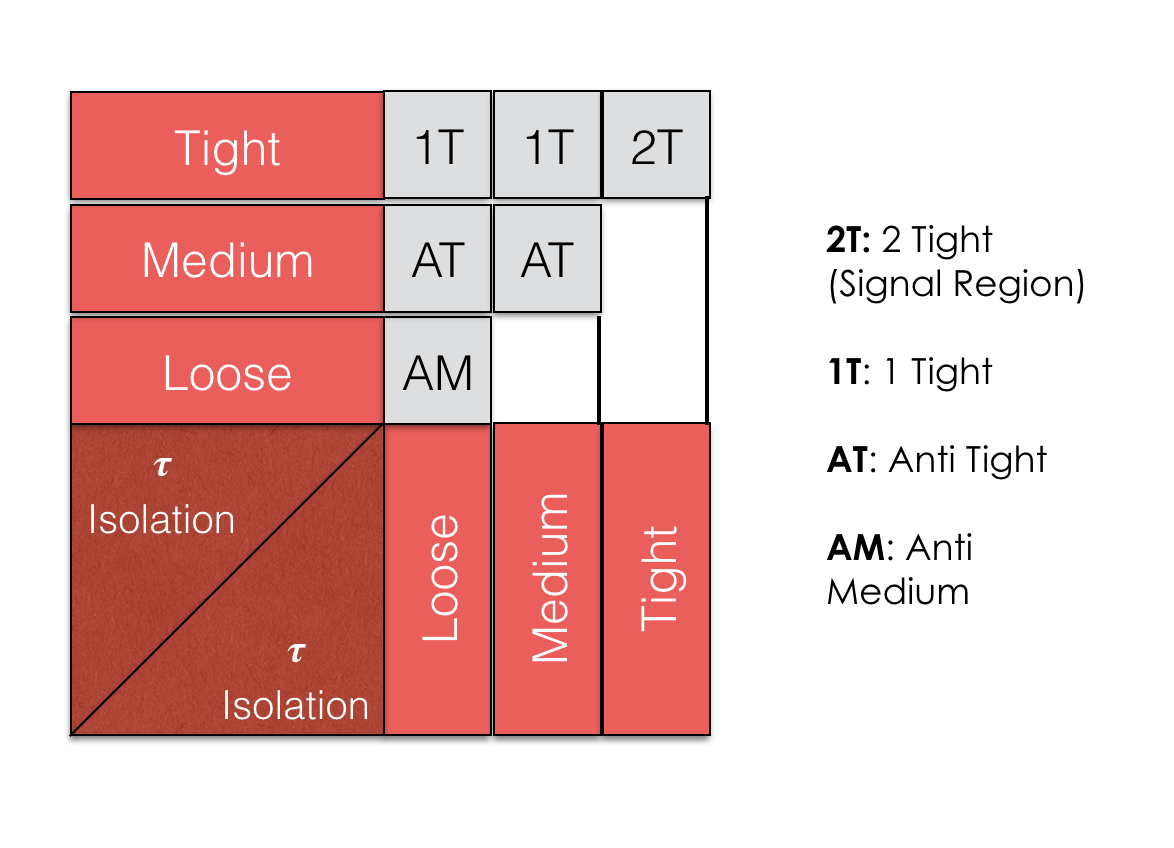
\includegraphics[width=0.75\textwidth]{PLOTS/diTauHadLSotherPlots/tauisoregions.png}
		\end{tabular}
		\caption{Definitions of the exclusive isolation region depending on the isolation of each of the $\hadtau$ where SR is Signal Region consisting of 2 tight isolated $\hadtau$, 1T is One Tight isolated Tau region consisting of one tight isolated $\hadtau$ and an additional medium or loose isolated $\hadtau$, AT is Anti Tight isolation region consisting of at least one medium isolated $\hadtau$ and an additional medium or loose isolated $\hadtau$,  AM is Anti Medium isolation region consisting of 2 loose isolated $\hadtau$}
		\label{fig:tauisoregions}
	\end{figure}
	
	\item \textbf{Inversion of the VBF Cuts}: We define a second dimension of exclusivity using VBF cuts described in \ref{sec:eventselection}. The regions are defined the following way:
	
	\begin{enumerate}
		\item VBF region: consisting of all the events that passed all VBF cuts previously mentioned;
		\item VBF inverted region: consisting of all the events that at least fails one of the VBF cuts previously mentioned;
	\end{enumerate} 
\end{enumerate}

Using these definitions, we define one signal region and 7 control regions, shown in Figure \ref{fig:crs}. In order to keep the QCD background contribution low in signal region and control region 2 an additional cut of  MET $ > $ 30 GeV is required. 

\begin{figure}[tbh!]
	\centering
	\begin{tabular}{cc}
		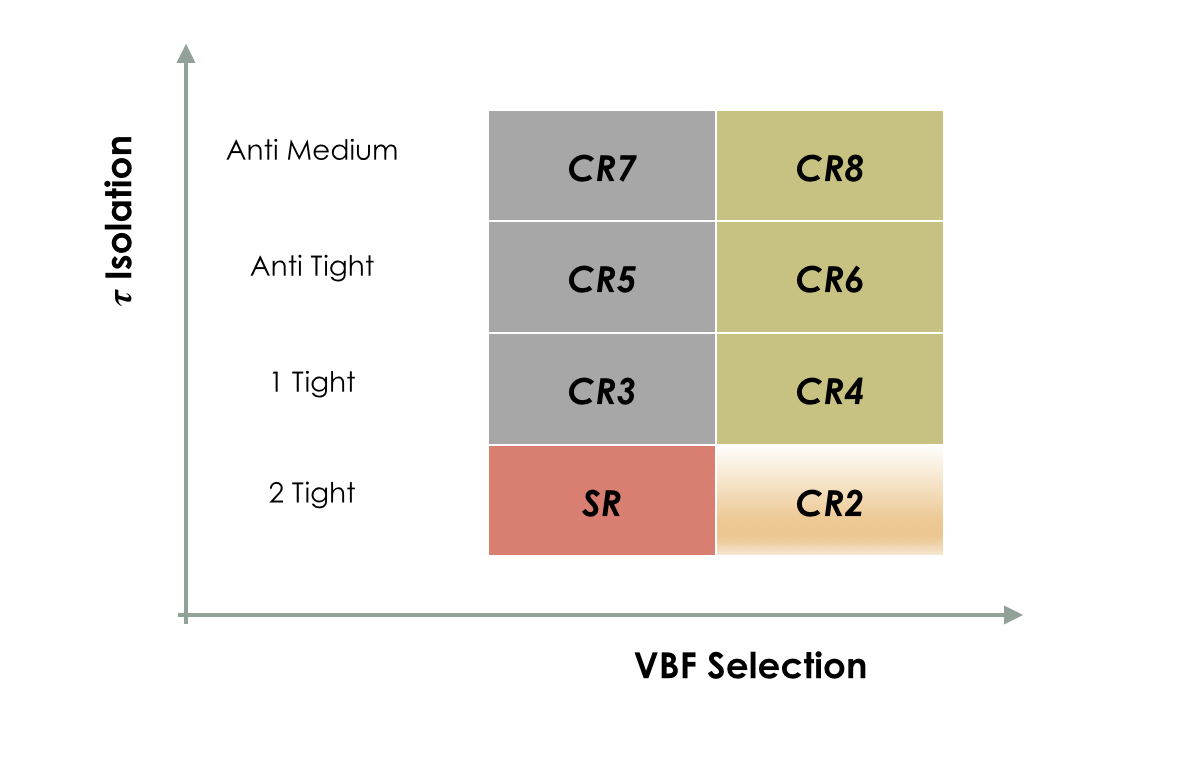
\includegraphics[width=0.75\textwidth]{PLOTS/diTauHadLSotherPlots/controlregions.png}
	\end{tabular}
	\caption{Definition of Signal and Control Regions using different $\hadtau$ isolation criteria and VBF selection.}
	\label{fig:crs}
\end{figure}

The signal and control regions are define under the assumption of central selection being orthogonal to VBF selection. Figure \ref{fig:LS_mjjshapestab_vs_tauiso_data} and \ref{fig:LS_mjjshapestab_vs_tauiso_mc} shows the results of the stability study of $M_{jj}$ shape distribution among different $\tau$ isolation sidebands for Data and MC. Further studies are shown in Section \ref{subsubsec:shapecomp}.

\begin{figure}[tbh!]
	\centering
	\begin{tabular}{cc}
		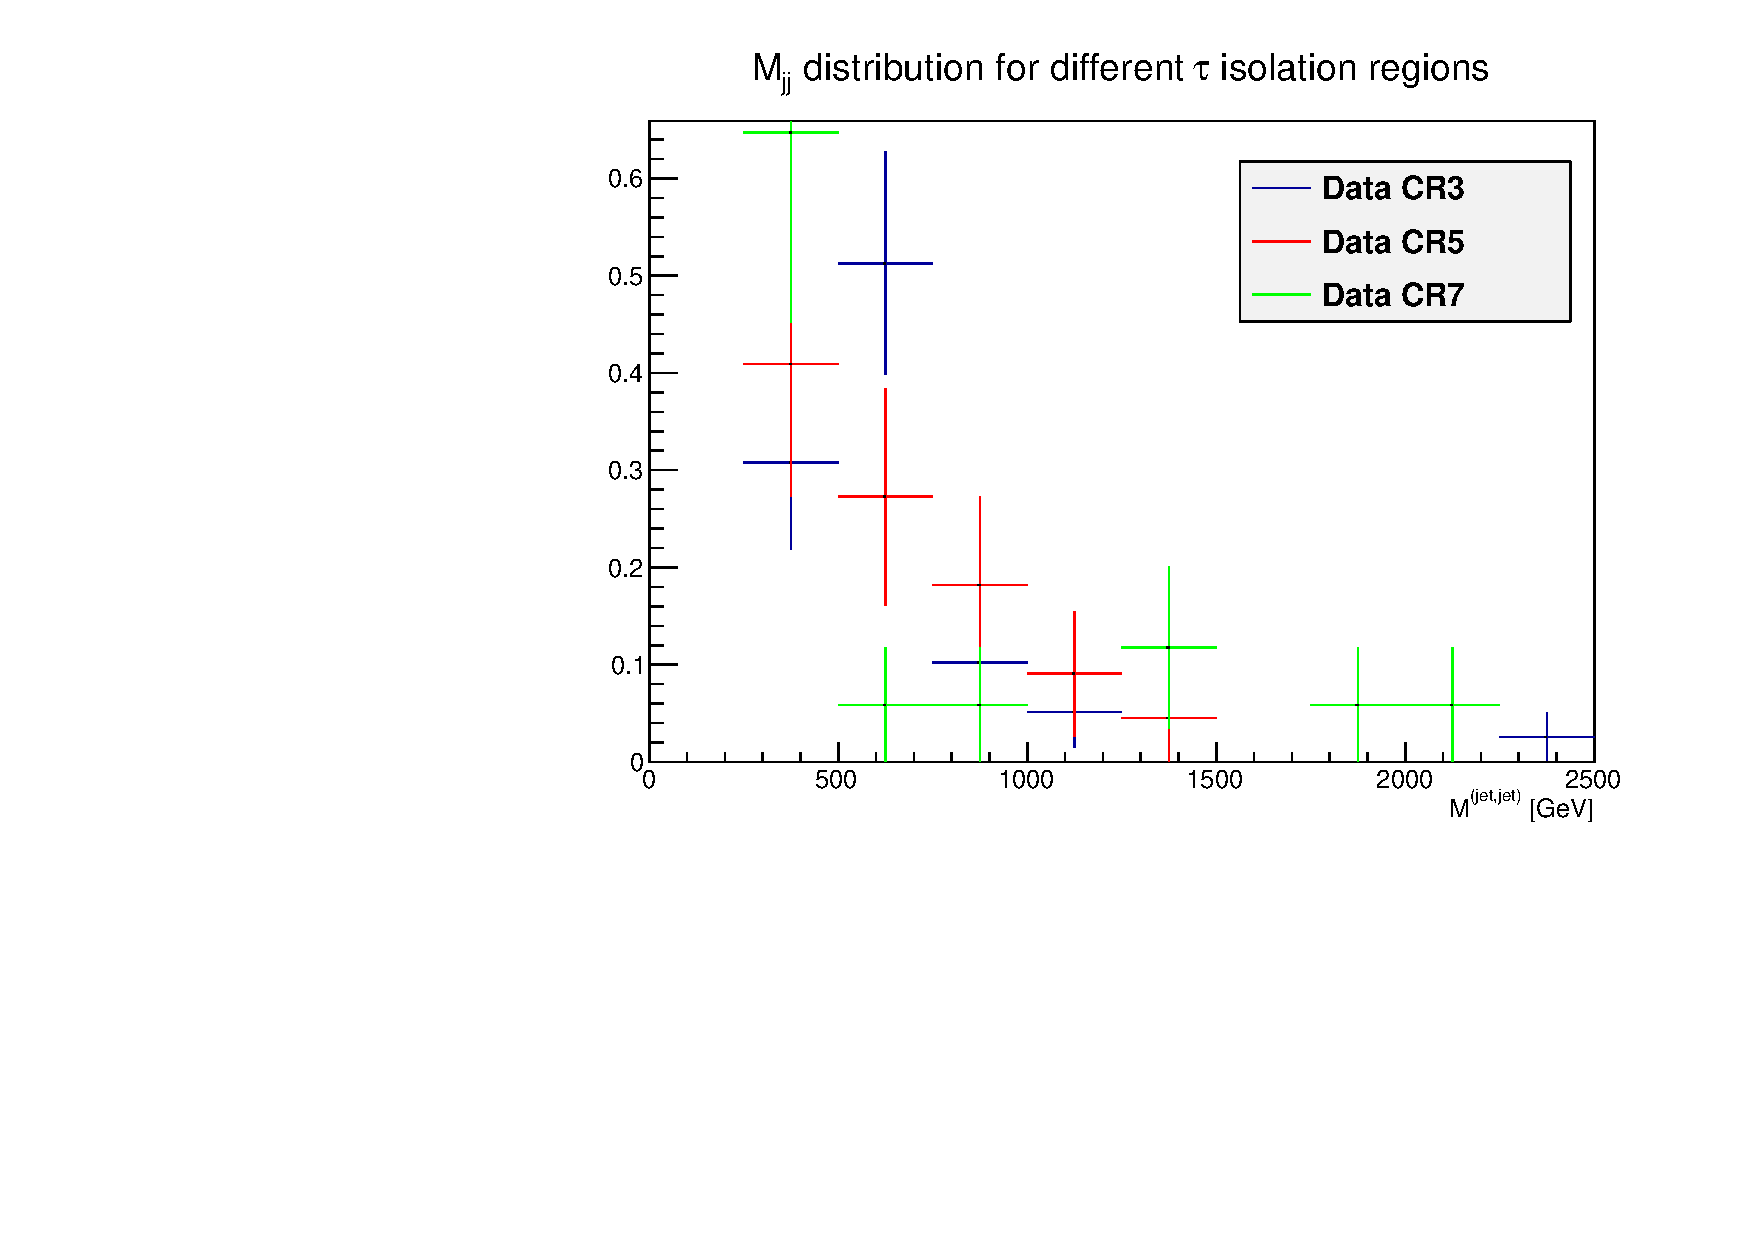
\includegraphics[width=0.75\textwidth]{PLOTS/diTauHadLSotherPlots/LS_mjjshapestab_vs_tauiso_data.pdf}
	\end{tabular}
	\caption{$M_{jj}$ shape comparisons among different $\tau$ isolation sidebands for Data (CR3, CR5, CR7)}
	\label{fig:LS_mjjshapestab_vs_tauiso_data}
\end{figure}

\begin{figure}[tbh!]
	\centering
	\begin{tabular}{cc}
		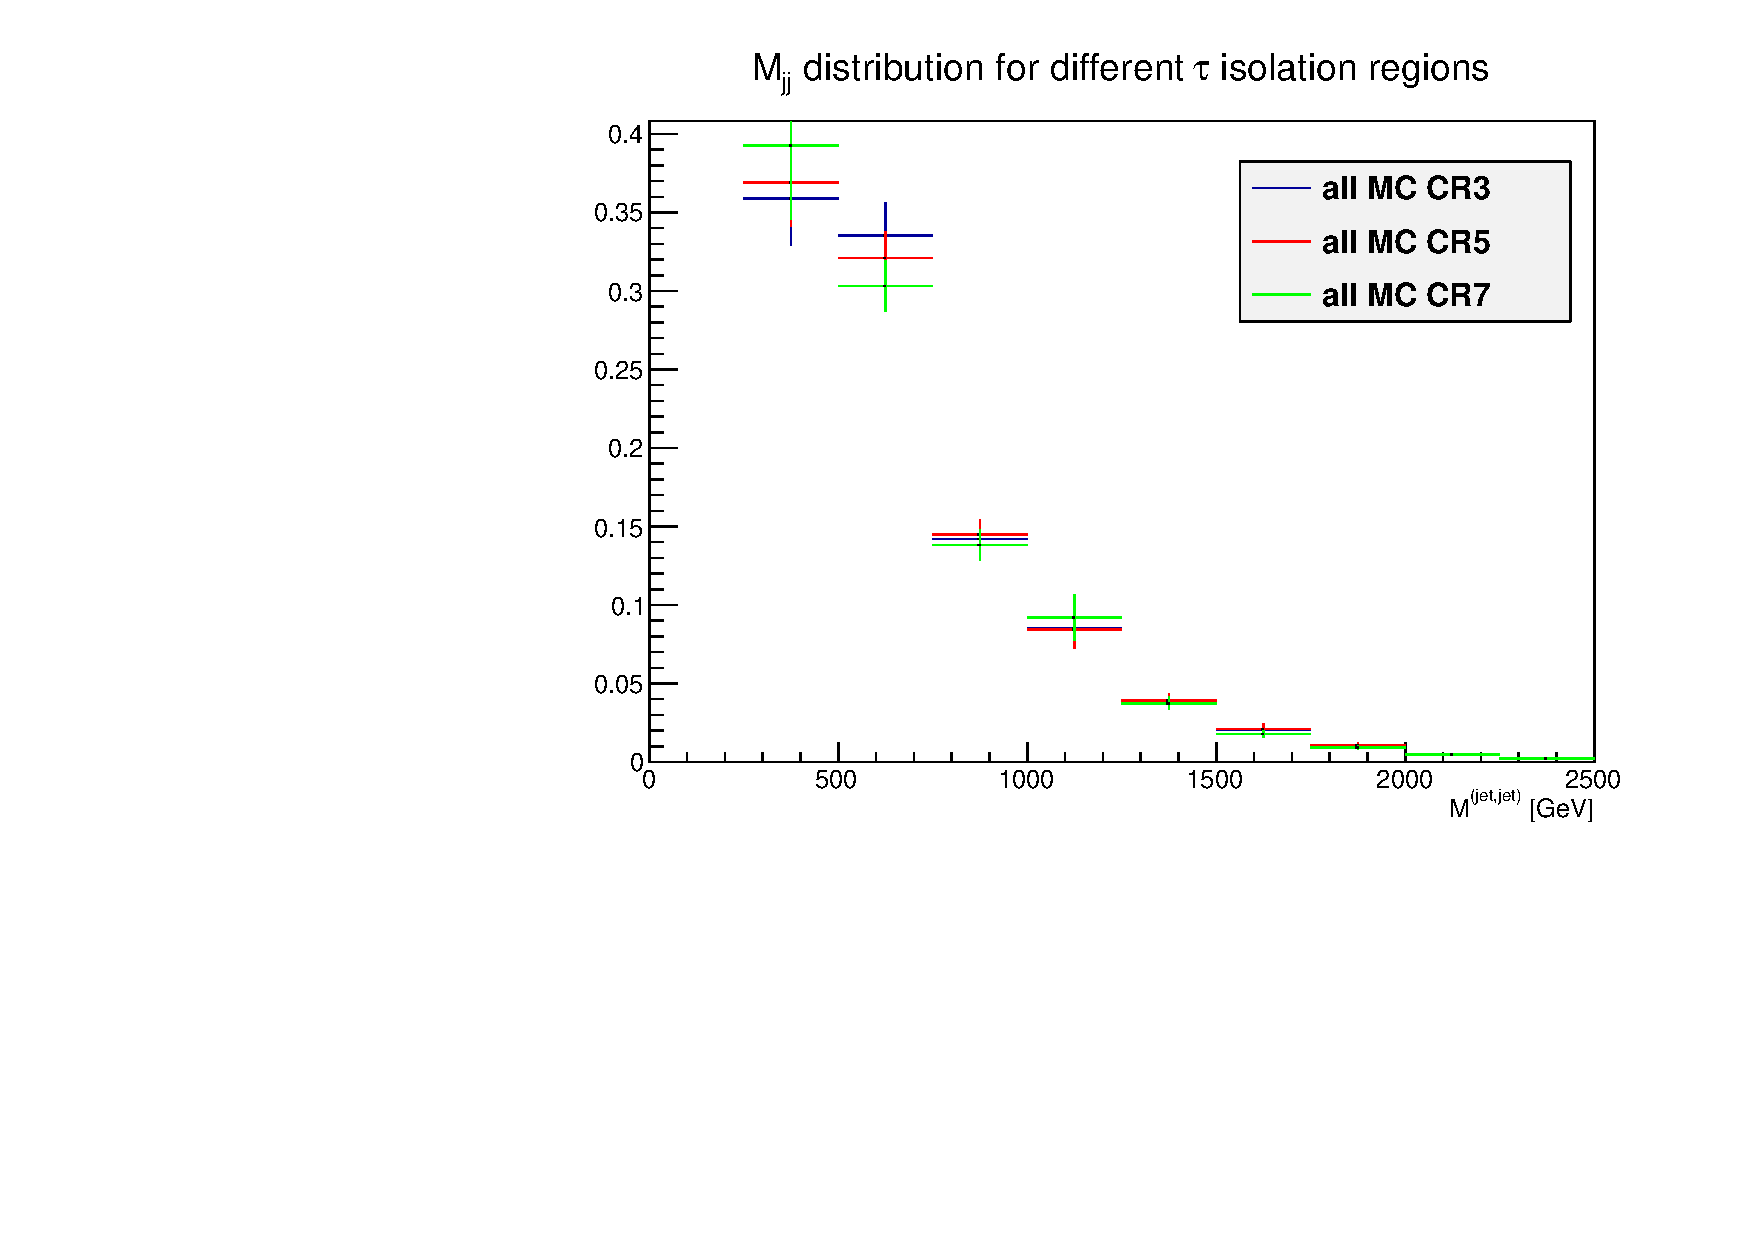
\includegraphics[width=0.75\textwidth]{PLOTS/diTauHadLSotherPlots/LS_mjjshapestab_vs_tauiso_mc.pdf}
	\end{tabular}
	\caption{$M_{jj}$ shape comparisons among different $\tau$ isolation sidebands for all MC contributions (CR3, CR5, CR7)}
	\label{fig:LS_mjjshapestab_vs_tauiso_mc}
\end{figure}

The estimation of the events in the signal region is done similarly to any other data driven ABCD method by counting the number of events in CR2 (two $\tau$ with tight isolation and inverted VBF selection criteria) and multiplying it with a proper conversion factor described in the following equation:

\begin{equation}
N^{QCD}_{SR} = \left( N^{DATA}_{CR2} - N^{\overline{QCD} BG}_{CR2} \right) * \left[ \frac{\epsilon^{QCD}_{VBF}}{1 - \epsilon^{QCD}_{VBF}} \right]
\label{eq:qcdbgpred}
\end{equation}

where $N^{QCD}_{SR}$ is the number of QCD events predicted in the signal region, $N^{DATA}_{CR2}$ is the number of data events in control region 2, $N^{\overline{QCD} BG}_{CR2}$ is the number of all non-QCD MC samples events in control region 2 and $\epsilon^{QCD}_{VBF}$ is the efficiency of VBF cuts in a given Tau isolation region derived with the following equation.

\begin{equation}
\epsilon^{QCD}_{VBF} = \frac {N^{DATA}_{VBF CR} - N^{\overline{QCD} BG}_{VBFCR}}{\left( N^{DATA}_{VBFCR} - N^{\overline{QCD} BG}_{VBFCR} \right) + \left( N^{DATA}_{\overline{VBF}CR} - N^{\overline{QCD} BG}_{\overline{VBF}CR} \right) }
\label{eq:vbfeff}
\end{equation}

where:

\begin{itemize}
\item $N^{DATA}_{VBF CR}$ is the number of the events in data for a given $ \tau $ isolation region and VBF region;
\item $N^{\overline{QCD} BG}_{VBFCR}$ is the number of all non-QCD MC events for a given $ \tau $ isolation region and VBF region;
\item $N^{DATA}_{\overline{VBF}CR}$ is the number of events in data in the same isolation Control Region but inverted VBF region;
\item $N^{\overline{QCD} BG}_{\overline{VBF}CR}$ is the number of all non-QCD MC events for a given $ \tau $ isolation region but inverted VBF region.
\end{itemize}

Three different predictions for the QCD contribution will be given, one for each pair of tau isolation control regions below the two tight isolation. The estimation of the QCD contamination, in the signal region,  as shown on Equation \ref{eq:qcdbgpred}, has two sources of systematics:  

\begin{itemize}
	\item[1]Uncertainty on the generated Monte Carlo samples used in the analysis
	\item[2]  Uncertainty on the stability of the VBF efficiency in regard to a loosening of the tau-identification as previously described in section \ref{sec:crsdef};
	\item[3] Uncertainty on the stability of the VBF efficiency in regard to a loosening of the \met cut, since the $\epsilon^{QCD}_{VBF}$ is calculated in CRs where no \met cut is applied.
\end{itemize}

\begin{table}[ht]
	\centering{
		%   \tabcolsep=0.05cm
		\begin{tabular}{| l | c | c | c |}
			\hline\hline
			Sample     &Events (SR)   &Events (CR2)     &Events (CR3)       \\ [0.5ex] \hline
			Data &$ - $    &$ 109$    &$ 39$     \\
			Drell-Yan &$ 0.037\pm0.015$    &$ 1.3\pm1$    &$ 0.042\pm0.0077$     \\
			VV &$ 0.11\pm0.065$    &$ 0.7\pm0.09$    &$ 0.035\pm0.017$    \\
			W+Jets &$ 0.53\pm0.04$    &$ 6.6\pm0.17$    &$ 0.83\pm0.055$    \\
			Single t &$ 0.036\pm0.0066$    &$ 0.25\pm0.017$    &$ 0.057\pm0.008$   \\
			\ttbar &$ 0.11\pm0.012$    &$ 1.4\pm0.051$    &$ 0.19\pm0.013$   \\
			Higgs &$ 0.0005\pm7.2e-05$    &$ 0.012\pm0.0048$    &$ 0.0029\pm0.0023$   \\
			QCD &$ 8.6\pm0.61$    &$ 54\pm1.2$    &$ 47\pm1.9$   \\
			\hline
			Total nonQCD MC &$ 0.83\pm0.079$    &$ 10\pm1$    &$ 1.2\pm0.06$   \\
			\hline\hline
		\end{tabular}
	}
	\caption{Number on events in SR, CR2, CR3 for data and all MC samples used for the estimation of $N^{QCD}_{SR}$}
	\label{table:CReventcount1} % is used to refer this table in the text
\end{table}

\begin{table}[ht]
	\centering{
		%   \tabcolsep=0.05cm
		\begin{tabular}{| l | c | c | c |}
			\hline\hline
			Sample   &Events (CR4)  &Events (CR5)     &Events (CR6)    \\ [0.5ex] \hline
			Data    &$ 737$  &$ 22$    &$ 312$      \\
			Drell-Yan    &$ 0.65\pm0.045$  &$ 0.002\pm0.00076$    &$ 0.029\pm0.0037$    \\
			VV   &$ 0.6\pm0.1$   &$ 0.0031\pm0.001$    &$ 0.045\pm0.015$   \\
			W+Jets    &$ 10\pm0.2$  &$ 0.081\pm0.0096$    &$ 0.89\pm0.034$      \\
			Single t   &$ 0.47\pm0.02$   &$ 0.011\pm0.00076$    &$ 0.1\pm0.0028$      \\
			\ttbar  &$ 2.5\pm0.059$   &$ 0.04\pm0.0024$    &$ 0.52\pm0.0095$      \\
			Higgs  &$ 0.012\pm0.0044$   &$ 2.7e-05\pm1.1e-05$    &$ 0.00018\pm2.2e-05$    \\
			QCD  &$ 3.4e+02\pm4$  &$ 19\pm0.68$    &$ 1.4e+02\pm1.6$    \\
			\hline
			Total nonQCD MC  &$ 15\pm0.24$ &$ 0.14\pm0.01$    &$ 1.6\pm0.038$    \\
			\hline\hline
		\end{tabular}
	}
	\caption{Number on events in CR4, CR5, CR6 for data and all MC samples used for the estimation of $N^{QCD}_{SR}$}
	\label{table:CReventcount2} % is used to refer this table in the text
\end{table} 

\begin{table}[ht]
	\centering{
		%   \tabcolsep=0.05cm
		\begin{tabular}{| l | c | c |}
			\hline\hline
			Sample      &Events (CR7)     &Events (CR8)  \\ [0.5ex] \hline
			Data     &$ 17$    &$ 184 $  \\
			Drell-Yan    &$ 0.0012\pm0.00057$    &$ 0.013\pm0.0021 $  \\
			VV   &$ 0.0011\pm0.00014$    &$ 0.033\pm0.016 $  \\
			W+Jets    &$ 0.036\pm0.0051$    &$ 0.35\pm0.015 $  \\
			Single t   &$ 0.0061\pm0.00045$    &$ 0.058\pm0.00087 $  \\
			\ttbar  &$ 0.022\pm0.00079$    &$ 0.32\pm0.0054 $  \\
			Higgs  &$ 4.9e-06\pm2.3e-06$    &$ 5.7e-05\pm1e-05 $  \\
			QCD  &$ 15\pm0.81$    &$ 1.1e+02\pm1.7 $  \\
			\hline
			Total nonQCD MC  &$ 0.067\pm0.0053$    &$ 0.77\pm0.023 $  \\
			\hline\hline
		\end{tabular}
	}
	\caption{Number on events in CR7 and CR8 for data and all MC samples used for the estimation of $N^{QCD}_{SR}$}
	\label{table:CReventcount3} % is used to refer this table in the text
\end{table} 

\begin{table}[ht]
	\centering{
		\tabcolsep=0.05cm
		\begin{tabular}{| l | c | c | c |}
			\hline\hline
			Variable     &One Tight region     &Anti-Tight region     &Anti-Medium  \\ [0.5ex] \hline
			$\epsilon^{QCD}_{VBF}$    &$ 0.05\pm0.008 $  &$ 0.066\pm0.014 $  &$ 0.085\pm0.02 $ \\
			$N^{QCD}_{SR}$    &$ 5.2\pm1 $  &$ 6.9\pm1.7 $  &$ 9.1\pm2.5 $ \\
			\hline\hline
		\end{tabular}
	}
	\caption{ Values for $\epsilon^{QCD}_{VBF}$ and $N^{QCD}_{SR}$ for different $ \tau $ isolation regions.}
	\label{table:VBFeffBKGprediction} % is used to refer this table in the text
\end{table}

Systematics for the simulation are estimated by scaling non-QCD contributions by $\pm50~\%$. A systematic error on $\epsilon^{QCD}_{VBF}$ is assigned by using the maximal variation among all $\epsilon^{QCD}_{VBF}$ measurements in different $\tau$ isolation regions with respect to its weighted mean. Similar procedure is done for the assignation of the $\epsilon^{QCD}_{VBF}$ coming from \met cut stability. All the statistical uncertainties are propagated accordingly. Tables \ref{table:CReventcount1} , \ref{table:CReventcount2} and \ref{table:CReventcount3} show the event counting for all the control regions previously defined for data and all MC samples. All the numbers except the ones coming from the QCD sample are used as input for the QCD background estimation method. For each of the 3 different $\tau$ isolation regions out of the signal region (1T, AT, AM) an independent measurements of $\epsilon^{QCD}_{VBF}$  and prediction for $N^{QCD}_{SR}$ is made. Due to low statistics in the $\tau$ isolation sidebands the final results will include uncertainties coming from the $\epsilon^{QCD}_{VBF}$ stabilities studies on MC shown in section \ref{subsec:stability}.



\section{Data Driven method validation}
\label{QCD_bg_pred_validation}

